\documentclass{article}
\usepackage{parskip}
\usepackage{amssymb,amsmath}
\usepackage{graphicx}
\usepackage{biblatex}
\bibliography{Improvise}

\begin{document}

\title{The Prisoner's Sonata: \\ \large Modeling Musical Improvisation with Game Theory}
\date{}
\author{Caroline Marcks, Andrew Mendelsohn, and Jayme Woogerd}
\maketitle


\section{Introduction}

In \emph{A Model of Performance, Interaction, and Improvisation}\cite{hudakberger95}, Paul
Hudak and Jonathan Berger outline a formal model of musical performance, interaction and
improvisation based on the idea that a full musical performance can be
understood as a set of complex, interrelated interactions.

To motivate this model, they observed that in any performance there exists
an interaction between a player and himself: throughout the performance,
a good musician will continuously make adjustments to his playing based
on what he is hearing from his own instrument. Likewise, in an ensemble
or orchestral performance, a player is necessarily affected by the
performance of each of the other players in the ensemble. Finally, each
player is working off his interpretation of the musical score
and, in the case where the players are improvising, the produced
performance may actually deviate wildly from what is given in the score.

In the paper, these interactions are termed \emph{mutually recursive
processes} where ``the recursion captures feedback {[}and{]} mutual
recursion captures the interaction between players''.\cite{hudakberger95} In
concrete terms, these relationships of interaction are defined
algebraically as:

\begin{verbatim}
    r = instr(player s r)
\end{verbatim}


where \texttt{r} is the realization, the music actually produced by a
player, and \texttt{s} is the score.  They then note that in the
context of improvisation, ``although the goal of those involved\ldots{}is generally one of cooperation, there is also a certain amount of
conflict.''\cite{hudakberger95}  Given this natural relationship of conflict and cooperation
between players in an improvisational scenario and the mathematical
model we can use to frame it, they suggest the application of \emph{game
theory}.

Grounded in this theoretical framework for how a music game might
work, this project set out to explore a new method of algorithmic music
composition. Thus, the goals of the project were:

\begin{itemize}
\itemsep1pt\parskip0pt\parsep0pt
\item
  Implement in Haskell the game theoretic model outlined in Hudak and Berger's
  paper
\item
  Produce a meaningful, new way of algorithmically generating music that
  resembles human improvisation
\item
  Allow for the implementation to be extended through user-defined ideas
  of payoffs, strategies and rules
\end{itemize}

\section{Background: Game Theory}

\subsection{Concepts}
Game theory is the study of strategic decision making, used to model
interactions between agents whose decisions affect each other. In
traditional game theory, a \emph{game} is a situation in which two or
more agents make decisions. The agents are called \emph{players} and the
decisions they make are \emph{moves}. The \emph{rules} of the game
define a set of legal moves available to each player for any
\emph{state} of the game. The algorithms that players employ to choose
moves at any game state are called \emph{strategies} and can either be
algebraically defined or non-deterministic. A player is said to be
playing an optimal strategy when it always results in her receiving her
maximum possible \emph{payoff} at the game's conclusion, where the
payoff is a quantified measure of the player's success. Game theory uses
\emph{game trees} to model the entire decision making process, where
each node contains the state of the game, and each branch is an event
that modifies that state.

\subsection{Experimental Game Theory}
Hagl is a domain-specific language embedded in Haskell that allows for
simple and modular definitions of experimental games.\cite{gametheorythesis, gametheory}  It provides easy interfaces for
defining what each of the above terms means in the context of a specific
game. Each game is an instance of a type class, which requires the
definition of a number of pieces.

\begin{verbatim}
    class GameTree (TreeType g) => Game g where
        type TreeType g :: * -> * -> *
        type State g
        type Move g
        gameTree :: g -> (TreeType g) (State g) (Move g)
\end{verbatim}

\texttt{TreeType}, \texttt{State}, and \texttt{Move} are associated
types defined in terms of \texttt{g}, the particular game. A \texttt{Game}
instance provides a \texttt{gameTree} function, which constructs the
game tree for the specific game. Hagl provides a number of operations
for interacting with the game values by examining internal tree nodes
and edges.

The \texttt{TreeType} must fit into Hagl's representation of a
\texttt{GameTree} as well. This game tree represents every possible
sequence of moves from an initial game state to all final states. Game
trees are rooted at the starting state, and each branch or edge
represents a possible move for a player or chance for an external event
to change the game state. Leaf nodes represent the final states,
associated with the payoffs for every player. Game trees may either be
\emph{continuous} or \emph{discrete}.  In discrete game trees, there
are a fixed number of edges and therefore a finite set of moves, while
in continuous trees the set of moves is potentially infinite and is
defined by a function from move to subtree.

When designing the \texttt{gameTree} function, one must consider the
\emph{information} each player has about the game state; this knowledge
may or may not be be shared amongst the players. When the players make
their decisions at the same time, we call this a \emph{simultaneous}
game and restrict the players' knowledge of the others' decisions until
all moves have been made and the game state updates en masse at the end
of a round.

\subsection{A formal treatment of
Tic-tac-toe}

As a brief example, consider the well-known game Tic-tac-toe.  The players
are the characters `X', and `O', who make their moves by placing their
mark on a 3 by 3 grid. The rules state that the players must alternate
turns. On each turn a player must put his mark in a previously
unoccupied cell. When three cells in a row are occupied by the same
player (horizontally, vertically, or diagonally), that player wins and
the game is over. If the board fills up before this can happen, the
result is a draw. Players each have knowledge of where both players have
moved on the board prior to the current turn (therefore, Tic-tac-toe is
not an example of a simultaneous game). Payoffs in this game are fixed:
1 for the winning player, -1 for the losing player, and 0 for each
player in the case of a draw. The first few levels of the game tree
might look like \emph{Figure 1} above.

\begin{figure}
\centering
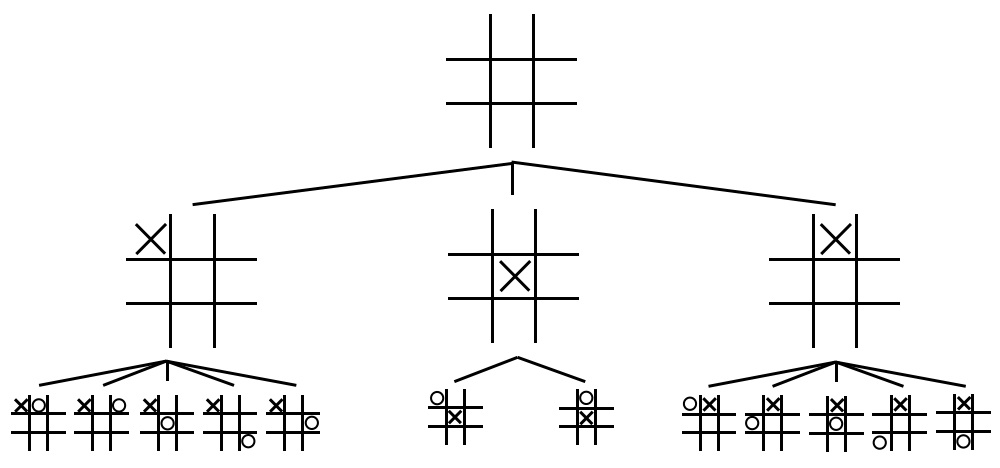
\includegraphics[width=90mm]{ttt.jpg}
\caption{Two levels of the Tic-tac-toe game tree}
\end{figure}

The first row models the options for player X's initial move.  The second row 
shows O's possible follow-up moves.

\section{Musical Improvisation as a
Game}

Given this general game theoretic framework, how do we then map the
fundamental components of a game to aspects of an improvisational
performance of two or more musicians?

\subsection{Moves}
For a musical game, moves take the form of fixed-duration, time-stamped
musical events.\cite{hudakberger95}  Rather than thinking of a player's full performance as a
sequence of notes, we imagine it as a sequence of musical events, that
is, a stream of his decisions of what and how to play at each
time-stamp.

Events must necessarily be both time-stamped and of a fixed-duration to
ensure that players make their decisions of what to play for each event
at the same time. Notes in the musical sense are associated with a given
duration, but consider a game in which one player begins playing a whole
note and the other a quarter.  When should we define the next decision
point at which the players can choose their next moves? When the second
player is ready to make another move, the first still has three more
beats to play. Thus, we break notes into events of fixed-duration and
allow a player to choose to extend the pitch of the previous event if he
or she desires to play a note of a longer duration.

In their paper, Hudak and Berger note that the formal model of musical interaction
``is limited to controlling an instrument's sound, for the purposes of
realizing fundamental parameters such as pitch in addition to more
subtle issues of articulation, dynamics and phrasing.''\cite{hudakberger95}  Indeed, in our
simple implementation, we focus solely on controlling pitch, ignoring
the more subtle parameters and keeping the players' instruments fixed.

\subsection{Payoff}
The payoff of the game, used to measure a player's success in the
performance, translates to a player's notion of musical aesthetic. This
is a measure of how good the musician considers the sound of his own
performance in the context of the whole piece. This preference is
unique to each player and may be defined along any axis of the musical
design space. The realm of musical aesthetic is practically infinite,
and a full discussion of music theory of this depth is well beyond the
scope of this paper.

\subsection{Strategy}
Each player in a musical game implements her own strategy, which
determines what she will play at any given point in the performance. In
a musical improvisational game, a strategy can be as simple as a player
adhering to her given score, never improvising at all.
Alternatively, a strategy can be more sophisticated.  It may take into account
past or anticipated payoffs, a player's own past moves or those of
another player, or some other musical strategy with the only restriction
that any move generated fall within those allowed by the
rules of the game.

For each individual, the goal of the game is to maximize his own
payoff. However, we note that unlike zero-sum games, which are purely
competitive, a musical game is more cooperative in nature. Indeed, there
exists some competition between players -- Hudak and Berger imagine two soloists
``vying for attention.''\cite{hudakberger95}  However, intuitively there is a point at which
trying to make the other player ``sound bad'' (i.e.~reduce his payoff)
has an equally deleterious effect on one's own performance. Therefore,
the best outcome for each player individually is likely to be one in
which the sum of their collective payoffs is also maximized.

\subsection{Game Tree}
We model this musical improvisational game with a discrete, simultaneous
game tree. We eliminate the possibility of chance from the tree: at
internal nodes, only a player's choices may affect the state of game.
Every edge represents a choice a performer can make to stick to or
deviate from the score. The tree represents the mutual recursion between
the players in that each player's decision depends on the previous
decisions of all other players.

\section{Improvise: our
implementation}

In order to implement music as a playable game, we must implement the
aforementioned components of games: moves, payoffs, and strategies. The
choices made here define the framework for the game itself, and
therefore, the range of music that can be produced from it.  Our 
implementations for some components are static and fixed, and others 
can change with each instance of an \texttt{Improvise} game.

\subsection{Static Components}
\subsubsection{Moves}
The first important piece is the \texttt{MusicMv}:

\begin{verbatim}
    data MusicMv = Begin  Pitch
                 | Extend Pitch
                 | Rest
\end{verbatim}

which defines a move as either a \texttt{Begin} of a \texttt{Pitch},
\texttt{Extend} of a \texttt{Pitch}, or a \texttt{Rest}. Each represents
a musical event of the game's defined smallest duration. Here again we make
the distinction between a \texttt{Begin} and \texttt{Extend} . A
\texttt{Begin} represents the onset or attack of the given pitch,
whereas an \texttt{Extend} is a continuation of the previous pitch
without a distinct onset. The difference lies in the following example:
Given a sequence of moves \texttt{{[}Begin p, Begin p{]}}, the sound
produced would be a note of length one unit followed by another note of
length one. There will be an audible separation of the two notes and a
distinct beginning of the second immediately following the termination
of the first. In contrast, the move sequence
\texttt{{[}Begin p, Extend p{]}}, would produce a note of twice the
duration with no audible onset beyond the first. The notes will sound as
one continuous event lasting two units. A \texttt{Rest} represents no
audible sound, simply one unit of silence.

The reasoning behind giving \texttt{Extend} a pitch is somewhat subtle. It is
necessary in our implementation for an \texttt{Extend} to directly
follow either a \texttt{Begin} or another \texttt{Extend}. In both
cases, the extension of the preceding note must contain the same pitch.
It is unclear then why \texttt{Extend} should be given a pitch at all,
as it should be simple enough to look back through the previous moves
until the most recent \texttt{Begin}, to which the extension is being applied, is
found. We found this to be slightly impractical later on when attempting
to write strategies and payoffs. The cost in storage of the
\texttt{Pitch} must be weighed against the cost in time of repeatedly
looking back to find it. This decision also lifts the burden from the
programmer when writing payoffs and strategies.

\subsubsection{State}
The next piece of the game implementation is the \texttt{Performer}:

\begin{verbatim}
    data Performer = Performer { realization :: [MusicMv]
                               , future      :: [MusicMv] }
\end{verbatim}

represents an individual player. The 
\texttt{realization} is
a list of musical events that have already occurred, i.e.~the player's
interpretation of the score thus far (most recent event first). The
\texttt{future} is a list of the upcoming events, i.e.~the remaining portion of
her score. Therefore, the whole performance is a \texttt{Performer} list, given by:

\begin{verbatim}
    type Performance = ByPlayer Performer
\end{verbatim}

A \texttt{ByPlayer a}, as defined in Hagl, is a list of \texttt{a} which
has length equal to the number of players in the game.

\subsubsection{Game Tree}
From here, we must design the generation of the tree to fit a few
requirements. First, it must keep a state in each node, and continually
modify that state as moves get played. Second, it must appear to players
that they are all making moves at once, despite the fact that a node can
only represent a move by one player. Third, it must have leaf nodes
populated with final payoff whenever the state makes it clear the game
is over. Finally, it must be efficient and expand as needed rather than
on first call of the function.

We use a recursive function to generate a discrete, simultaneous game tree and take advantage of
lazy evaluation to prevent the whole tree from being expanded at
once. Nodes that are never explored in the process of the game will
not be expanded at all. To enforce the stipulation in a simultaneous
game that players be ignorant of each others' moves during a round, 
we build out the game tree by accumulating all of the moves for
the round in a list and do not update the game state until every player
has made her decision. This accumulating list of moves is never seen by
a player's strategy, but only used in game tree generation, so is safe.

\subsection{Dynamic Components}

It is desirable to modularize those aspects of the game that we identify
as particular to a unique game execution. Most obviously, we will want
to experiment with different initial scores, that is, a user should be
able to play an \texttt{Improvise} game with any song of his choosing.

We wrap these dynamic quantities in the type \texttt{Improvise}:

\begin{verbatim}
    data Improvise = 
        Imp { state    :: Performance
            , payoff   :: Performance -> Payoff
            , playable :: Performance -> PlayerID -> [MusicMv]}
\end{verbatim}

Here a user may define the number of players and their initial scores in
\texttt{state}. In most games, prior to execution, each
\texttt{Performer} will have a \texttt{future} loaded with an individual
score as a list of \texttt{MusicMv} and an empty \texttt{realization}.
In our implementation, we provide infrastructure for rendering a list of
MIDI files of each player's score into an initial state of type
\texttt{Performance}.

\subsubsection{Payoff}
\texttt{Imp} also requires a function \texttt{payoff} that generates a 
Hagl \texttt{Payoff} matrix for any given game state.  At various times in the development of
\texttt{Improvise}, it was suggested that payoff be generated based on tempo
changes, sequences of notes, or even by more sophisticated schemes
derived from common jazz improvisational techniques. Recognizing the
fact that there are practically an infinite number of dimensions upon which to
judge musical aesthetic, it is critical that payoff generation has the
most general type possible.

In our implementation, we modeled an extremely simple idea of how a
player might judge the sound of his performance: that of pitch
intervals, the relative distance on the scale between two notes. In
Western music theory, some pitch intervals are generally considered to
sound ``consonant'', or pleasing - the classic example is that of a
major-third, two notes that are four semitones apart on a scale. Other
intervals, like the augmented-fourth (six semitones apart), may be
termed ``dissonant'' and are considered to cause tension in a piece.
Most pieces will use a mix of consonant and dissonant sounds to
alternately build and resolve tension.

For an \texttt{Improvise} game using the \texttt{intervalPayoff} function, this
means that each player provides his own interval preferences: an
association list of intervals (as a integer number of half-steps, or
semitones) and a \texttt{Float}, representing the relative value the player
places on playing that interval. Positive payoffs denote favorable
intervals for the player, while negative payoffs signify undesirable
ones.

Intervals not included in the list have a baseline value of zero for the
player; an empty interval preference list denotes a player who values
all intervals equally. We also distinguish the ``top'' player, playing
the higher note of the interval from the ``bottom'' player playing the
low note by allowing both positive and negative intervals. For example a
player with the preferences \texttt{{[}(4, 4.0), (-4, 2.0){]}} always
values major-thirds in a piece, but prefers to be the bottom player. The
idea is that if two players both have positive values for the same
interval, they will collude to play that interval more often.
Alternatively, a mix of positive and negative payoffs for a given
interval results in a more competitive relationship between players.

\subsubsection{Rules}
Finally, \texttt{playable} is a function for generating the legal moves
for a given player for any state of the game. 
For our studies, we defined a simple \texttt{playable}
function derived from the player's score: legal moves are those within a
set number of semitones away from the pitch given in the score. We
called this a ``range-limited'' move generation scheme. To make the
scheme slightly more sophisticated, we also allowed players to ``look
back'' at their most recently played note and play pitches within a
range around it as well. Players always have the option of
resting (emitting no sound) but we also stipulate that an \texttt{Extend} move is
only legal following a previous \texttt{Begin} or a previous \texttt{Extend}, never after
a \texttt{Rest}.

This \texttt{playable} function is fairly naive in the realm of music
improvisation and many other more realistic schemes have been suggested.
Given the generality of the \texttt{playable} function in the
implementation of \texttt{Improvise}, it should be possible to generate moves
based on other musical attributes of the piece.

\subsubsection{Strategies}

Hagl comes prepackaged with a classic game theory strategy
called \texttt{minimax}, in which a player simultaneously endeavors to
maximize his own payoff and diminish that of his adversary. To more
closely model the cooperative nature of a musical game, we implemented a
variation on this strategy, which we called \texttt{maximize}. In this
strategy, the player whose turn it is calculates an intermediate payoff
for each of his possible moves. This payoff is \emph{intermediate} because it is
not necessarily indicative of the final payoff.  From these intermediate payoffs, we pick the three nodes that yield the best payoff, and explore those nodes by
recursively calling the same maximize strategy for the next player. The
recursive algorithm continues until the bottom of the tree or a defined
depth limit, at which point, the player who began the exploration
considers the three payoffs at every level, and choose the maximum from
these.

Rather than immediately choosing the move that yields the highest intermediate payoff at every node, this strategy explores the tree by expanding out three nodes at a time.  We justify this by noting that a player cannot know how another player's decision in the future will affect his final payoff unless he explores the game tree.  Making an optimal move now may cause him to fall into a bad situation in the future.  On the other hand, a sub-optimal move now may open up a branch in the tree that ultimately yields him a higher final payoff.

\subsection{The State Space}

The design decisions made throughout the implementations of the above
dynamic components are centered around the state space. The size of a
tree grows exponentially with its branching factor. This means that if
each player makes \emph{n} decisions each from \emph{m} choices,
there are on the order of \emph{m\^{}n} nodes in the tree. The decision
to limit the range of possible pitch deviation from the score in the
\texttt{limitByRange} function aims to limit \emph{m}, while the depth
limit \texttt{maximize} aims to limit \emph{n}. If one was to make
every note on the piano legal in every context, the strategies may
explore 60 million game states within four
decisions. Our strategies take advantage of the lazy
evaluation of the game tree, and limit the branching factor by
limiting possible moves from each state. All further implementations of
strategies and \texttt{playable} should keep these factors in mind,
though we have kept these as dynamic parameters as the
willingness to allocate computational resources in the pursuit of good
improvisation may vary from person to person.

\section{Case Studies}

In this section we will walk through examples that illustrate some of
the capabilities of the \texttt{Improvise} game. The dynamic components used in
the examples are fairly straightforward and should serve to demonstrate
what can be accomplished with a basic strategy, payoff, and move domain.
For these examples, we will often refer to a payoff function
\texttt{pay} defined as follows:

\begin{verbatim}
    prefs1 = [(-3, 2), (-5, 2), (5, 2), (3, 2)]
    prefs2 = [(5, 1), (3, 1)]
    pay = intervalPayoff [prefs1, prefs2]
\end{verbatim}

As a reminder, this uses the association lists of intervals and preference
weights to generate a payoff matrix for each final state.

The two strategies showcased are \texttt{maximize pay}, which uses
our maximize strategy given the payoff function, and
\texttt{justTheScore}, which as its name indicates, plays the original
score.

The \texttt{playImprovise} function used to execute these games takes
all the dynamic pieces we previously discussed:

\begin{verbatim}
    playImprovise :: 
         (Performance -> Payoff)  --payoff function
      -> Performance              --starting score
      -> (Performance 
            -> PlayerID 
            -> [MusicMv])         --playable moves
      -> [Hagl.Player Improvise]  --players in the game (strategies)
      -> IO ()
\end{verbatim}

\subsection{``Mary Had a Little Lamb''}

In this first example we use ``Mary Had A Little Lamb'' as our starting
score for both players.

\begin{verbatim}
    playImprovise (intervalPayoff [prefs1, prefs2])
            ByPlayer [mary, mary]
            (limitByRange 2)
            [justTheScore, (maximize pay)]
\end{verbatim}

Below is the musical output of this example on the left as a list of
moves, annotated with the intervals and payoffs for each player on the
right.

\begin{verbatim}
["Mr. Score ", "Missus Maxine “]  Interval1 Payoff1 Interval2 Payoff2
[Begin  (A,4),  Begin  (A,4)  ]     0               0        
[Extend (A,4),  Extend (A,4)  ]     0               0        
[Begin  (G,4),  Begin  (G,4)  ]     0               0        
[Extend (G,4),  Extend (G,4)  ]     0               0        
[Begin  (F,4),  Begin  (F,4)  ]     0               0        
[Extend (F,4),  Extend (F,4)  ]     0               0        
[Begin  (G,4),  Begin  (E,4)  ]     -3      2       3       1
[Extend (G,4),  Extend (E,4)  ]     -3      2       3       1
[Begin  (A,4),  Begin  (Fs,4) ]     -3      2       3       1
[Extend (A,4),  Extend (Fs,4) ]     -3      2       3       1
[Begin  (A,4),  Begin  (Fs,4) ]     -3      2       3       1
[Extend (A,4),  Extend (Fs,4) ]     -3      2       3       1
[Begin  (A,4),  Begin  (Fs,4) ]     -3      2       3       1
[Extend (A,4),  Extend (Fs,4) ]     -3      2       3       1
[Extend (A,4),  Extend (Fs,4) ]     -3      2       3       1
[Extend (A,4),  Extend (Fs,4) ]     -3      2       3       1

Payoffs:
[20, 10]
\end{verbatim}

Going through this output, we see that at first both players choose to
play in unison, both following the score they were given. This is due to
the limited range by which they are allowed to deviate from the score.
To this point, they have not had an opportunity to produce any intervals
of any worth in terms of payoff. However, when we reach the 7th move, we
see Player 2 play an E below Player 1's G. The interval from Player 1's 
perspective is -3 as the move from a G to an E is down 3 half-steps. 
Conversely, the interval from Player 2's perspective is an E to a G which is 
an upward distance of 3 half-steps.  Player 1 values the interval -3 at a 
payoff of 2, while Player 2 values their interval, 3, at 1.

We can see that for all of the following moves, the intervals produced
are exactly the same. This is quite logical given the input to the game.
Looking back at \texttt{prefs1} and \texttt{prefs2}, we can see that Player 1 and Player 2
have both achieved the maximum payoff possible,
However, both players give equal weight to a 5 (or -5) interval as +/-3,
so why would Player 2 not choose to produce any? This turns out to be due
to the tie-breaking in the \texttt{maximize} strategy. We chose to have ties in
payoff broken by playing the note closest to the original score. This
prevents players from deviating further and further on each successive move,
creating notes in entirely different registers that do not remotely
resemble the score. Consequently, because Player 1 plays only the score,
intervals of 3 half-steps are by definition closer to the score than
those of 5 half-steps.

Though the choices made in terms of payoffs for this example are rather
simple and not necessarily the most meaningful for producing complex or
interesting music, they serve to illustrate the functionality of the
preference-based payoff system and the effectiveness of the \texttt{maximize}
strategy.

The example preferences used could be expanded to include more intervals, or even
the whole range of -12 to +12.  Additionally, a player can assign a relative
preference between different intervals by assigning them different weights.  
For example, if we doubled the weight of 5 and -5 in
the above preferences, it is likely we would have seen more of them in the
output. Though ties are broken by playing closest to the score, these
payoffs would not create a tie, there would be a clearly superior move
available according to the payoffs.

\subsection{``Don't Stop Belivieving''}

While "Mary Had a Little Lamb" produces interesting and pleasing results,
it is not often that two players start out playing and improvising from
the same score. What happens in a more realistic scenario, where they're
already playing a pleasing harmony? We tested this with the first few
measures of ``Don't Stop Believing'' by Journey.

\begin{verbatim}
    playImprovise pay 
        ByPlayer [DontStopMiddle, DontStopBass]
         (limitByRange 2) 
        [justTheScore, maximize pay]
\end{verbatim}

Once again, we have Player 1 adhering to the score while Player 2
improvises, using the same payoff function and set of preferences as
above. However, because these players are already harmonizing, 
even without any improvisation, they already achieve a positive payoff
of {[}16,4{]}.  However, with improvisation, they
have a payoff of {[}8,15{]}, and the realization sounds similar, but
with a slightly different bass line. Player 2 has kept in mind
a goal of making the whole performance better -- the cumulative payoff is 23
rather than 20 -- while still working to maximize his own payoff according to his preferences.

\section{Conclusion}

The field of algorithmic music generation is a relatively new and
growing one. A multitude of tools and methods exist, each employing a
different model for music and its creation. While many of these tools
are quite sophisticated and capable, none appear to implement a game
theoretic model. The model used in \texttt{Improvise} represents an approach
that more closely models the way humans make decisions and interact in
music. It also offers opportunity for near-infinite customization and
extension. Customized payoffs and strategies can be easily integrated to
produce music according to any definition of musical aesthetic and run
on any score. Because this work is in a largely unexplored area, there
is much room for expansion and alternative representations.

It is natural to model a music game discretely, as typically there are a finite number of notes a person would consider playing.  However, in a continuous game tree, rather than selecting moves from
a finite set of edges at every node, a player can "ask" the tree
whether a move from a given node is acceptable.  This may
prove an interesting way to represent a musical game, as players do typically
have a sense of what notes would sound good, and do not need to explore
the tree in order to find them. This representation could heavily limit the explored
state space depending on the adventurousness of the strategies.
This would involve a nearly complete reimplementation of this work,
as the game tree and representation of legal moves are what provide the
structure for the current formulation of the game.

There is much work to be done in how to define payoff calculations. 
Calculating a payoff based on preferences of intervals is
simple, and it is already widely acknowledge that there are intervals
that sound more pleasing than others. However, the aesthetic of complete 
pieces of music may be more accurately based on ideas of repetition and
variation or rates of consonance to dissonance than on harmonies alone.
These types of calculations are possible, but involve a much more
specific identification of the aesthetics of music, which cannot be 
universally defined. This project did not aim to explore those areas, but it 
may be an area for future exploration by those with technical
backgrounds in music theory.

Finally, we see many opportunities to further explore strategies suitable for an 
improvisational game.  None of the strategies implemented in this project 
took advantage of the fact that in Hagl a strategy is implemented as a state 
monad transformer, and so is capable of maintaining awareness of musical  
repetition or variation. We suspect that a stateful strategy of this kind
is computationally feasible as long as we limit the exploration of the game tree, and we look forward to pursuing this idea in the future.

\section{Acknowledgements}

We'd like to acknowledge Paul Hudak, Jonathan Berger and Eric Walkingshaw, without whose work
this project would not have been possible.  We'd also like to thank Norman 
Ramsey for his guidance and support and our Advanced Functional
Programming classmates for the genial class atmosphere throughout the semester.

\printbibliography
%\bibliographystyle{abbrv}
\end{document}
